%% CAPITULO 4
\hypertarget{estilo:capitulo}{}
\chapter{ANÁLISES E RESULTADOS DA ASSIMILAÇÃO DE \-PRE\-CI\-PI\-TA\-ÇÃO}

\section{Resultados}
\label{ss:resultados}

Nesta dissertação de mestrado foram realizados dois experimentos de assimilação de dados de precipitação, dos quais um foi denominado CFD$\_$SAP, representando o experimento de controle. Este experimento faz uso do filtro digital original do modelo EtaWS e não assimila os dados de precipitação do TRMM. O segundo experimento, denominado CFD$\_$CAP, também faz uso do filtro digital do modelo EtaWS e assimila os dados de precipitação do TRMM. Em ambos os experimentos foram assimilados dados provenientes do GTS. A distribuição espacial típica destes dados pode ser vistas na figura 1.2 do Capítulo 1.

Na análise dos resultados da assimilação de precipitação os experimentos denominados CFD$\_$SAP e CFD$\_$CAP, por mera simplicidade, serão renomeados para apenas SAP e CAP, respectivamente. Para a validação destes experimentos, foram utilizados os dados de precipitação observada do SALLJEX para o período de Janeiro de 2003. Foram feitas comparações subjetivas através da análise das diferenças dos campos de precipitação entre os experimentos e comparações objetivas (avaliação do skill) com o cálculo do Viés, Erro Quadrático Médio (EQM) e Correlação de Anomalia (CA) dos campos usuais de avaliação do skill. Estes campos são: ventos zonal e meridional, altura geopotencial, umidade relativa, temperatura do ar em 850, 500 e 250 hPa, além de água precipitável (integrado na vertical).

Para o cálculo do Viés e do EQM, foram consideradas as previsões de 6, 12, 18 e 24 horas dos experimentos SAP e CAP. Foi considerada também a Reanálise 2 do NCEP/DOE como grade de destino na qual os experimentos foram interpolados. Para o cálculo da Correlação de Anomalia, foram consideradas, além das previsões de 6, 12, 18 e 24 horas e da Reanálise 2 do NCEP/DOE, uma climatologia de 50 anos obtida a partir das previsões do modelo global T126L28 do CPTEC, interpolada para a grade do Eta 20 km. 
Em todos os cálculos, interpolou-se a grade dos experimentos e da climatologia na grade da Reanálise 2 do NCEP/DOE.

Os valores apresentados nos gráficos de Viés, EQM e CA representam a média dos valores dos campos no período de 17 a 29 de Janeiro de 2003. Foi desconsiderado o período de 02 a 16 de Janeiro de 2003, por ter-se reservado este como spin-up dos experimentos.

\subsubsection{Avaliação Estatística (Skill)}

Para o cálculo o Viés (equação 4.1), calculou-se as diferenças entre os campos de cada experimento considerado em relação à Reanálise 2 do NCEP/DOE. A seguir foi calculada a média do campo para o domínio de 50.2ºS 10ºN e 83ºW 25.8W, respeitando-se cada saída do modelo 0, 6, 12, 18 e 24h. 0h Indica o valor da análise e 6h o valor do first guess. Os gráficos são mostrados a seguir para as seguintes variáveis: Altura Geopotencial, Vento Meridional, Vento Zonal e Temperatura Absoluta. As colunas da esquerda representam o horário sinótico de 00Z, as colunas da direita o horário das 12Z. A primeira linha apresenta os resultados para o nível das 850 hPa, a segunda linha para o nível de 500 hPa e a terceira linha, para o nível de 250 hPa. O cálculo do EQM (equação 4.2) foi feito com base nos valores calculados do Viés. Para isso, tomou-se o quadrado as diferenças entre as previsões dos experimentos e a Reanálise. Para o cálculo da CA (equação 4.3), foram calculadas as anomalias dos experimentos (SAP e CAP) e a anomalia da Reanálise, conforme a equação 4.3.

\begin{equation}
Vies=E_{i}-R_{i}
\label{form10}
\end{equation}

\begin{equation}
EQM=(E_{i}-R_{i})^{2}
\label{form11}
\end{equation}

\begin{equation}
CA=\frac{\sum_{i=1}^{5}\{[(E_{i}-C)-\overline{(E_{i}-C)}]*[(R_{i}-C)-\overline{(R_{i}-C)}]\}}{\sqrt{\sum_{i=1}^{5}[(E_{i}-C)-\overline{(E_{i}-C)}]^{2}*\sum_{i=1}^{5}[(R_{i}-C)-\overline{(R_{i}-C)}]^{2}}}*100
\label{form12}
\end{equation}

Onde:

\begin{itemize}
\item $E$: representa um dos experimentos (SAP ou CAP);
\item $R$: representa a Reanálise 2 do NCEP/DOE;
\item $C$: representa a Climatologia;
\item $E-C$: representa a anomalia dos experimentos (SAP ou CAP);
\item $\overline{E-C}$: representa a média da anomalia dos experimentos (calculada com base no número de dias de avaliação);
\item $R-C$: representa a anomalia da Reanálise;
\item $\overline{R-C}$: representa a média da anomalia da Reanálise (calculada com base no número de dias de avaliação).
\end{itemize}

O índice $i$, varia de 1 a 5 e indica o tempo de previsão 0, 6, 12, 18 e 24 horas. No caso da reanálise, este índice indica a análise correspondente à hora de previsão do experimento. Para a climatologia, este índice não varia, visto que se utiliza um valor fixo para a hora sinótica avaliada (00Z e 12Z).

A seguir, são apresentados os resultados encontrados com o cálculo do skill do modelo EtaWS em relação à Reanálise 2 do NCEP/DOE.

Na \autoref{fig09} apresenta-se o Viés, EQM e CA da altura geopotencial para os horários das 00Z (coluna da esquerda) e 12Z (coluna da direita) para as previsões de 0 a 24 horas, no nível de 850 hPa. No geral nota-se que o experimento CAP apresenta resultados um pouco melhores no horário das 00Z durante 0 e 12 horas de previsão (figuras da coluna da esquerda) do que no horário das 12Z. No entanto, às 12Z (figuras da coluna direita) nota-se que entre 12 e 18 horas de previsão o experimento CAP apresenta resultados um pouco melhores. Isso pode ser devido ao fato de que às 12Z a quantidade de observações sinótica é um pouco mais abundante do que às 00Z. Além disso, este resultado indica que o modelo se ajustou aos dados de precipitação assimilados, se comparado com o viés presente em 6 horas de previsão e em comparação com o experimento de controle SAP, que neste mesmo horário apresenta viés quase igual a zero. Em relação ao desempenho, embora os valores de CA se apresentem aquém em relação ao que se conhece do modelo operacional Eta do CPTEC - mas considerando-se a metodologia apresentada, nota-se que o desempenho do experimento CAP, na média, foi melhor no horário das 12Z do que às 00Z. Novamente, isto pode ser devido ao fato de haver uma maior abundância de dados sinóticos assimilados na análise das 12Z, o que levou o modelo a se ajustar mais rapidamente aos dados de precipitação assimilados pelo EtaWS.

\begin{figure}[!hbp]
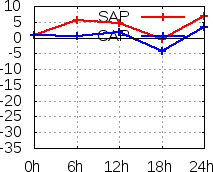
\includegraphics[height=5.5cm]{./figs/VIES850zgeo0Z.png}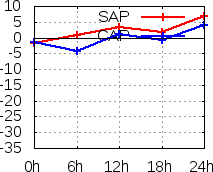
\includegraphics[height=5.5cm]{./figs/VIES850zgeo12Z.png}
\includegraphics[height=5.5cm]{./figs/EQMzgeo0Z.png}\includegraphics[height=5.5cm]{./figs/EQMzgeo12Z.png}
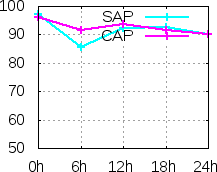
\includegraphics[height=5.5cm]{./figs/CA850zgeo0Z.png}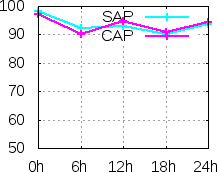
\includegraphics[height=5.5cm]{./figs/CA850zgeo12Z.png}
\caption{Viés, EQM e CA para a variável altura geopotencial em 850 hPa. A coluna da esquerda mostra os valores das medidas para o horário das 00Z. A coluna da esquerda mostra os valores das medidas para o horário das 12Z.}
\label{fig09}
\end{figure}

A próxima figura (\autoref{fig10}) mostra os valores dos índices estatísticos para a altura geopotencial no nível de 500 hPa.

\begin{figure}[!hbp]
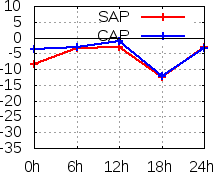
\includegraphics[height=5.5cm]{./figs/VIES500zgeo0Z.png}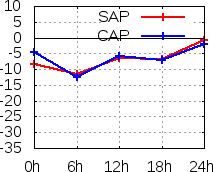
\includegraphics[height=5.5cm]{./figs/VIES500zgeo12Z.png}
\includegraphics[height=5.5cm]{./figs/EQMzgeo0Z.png}\includegraphics[height=5.5cm]{./figs/EQMzgeo0Z.png}
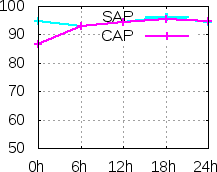
\includegraphics[height=5.5cm]{./figs/CA500zgeo0Z.png}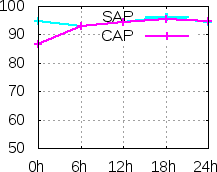
\includegraphics[height=5.5cm]{./figs/CA500zgeo0Z.png}
\caption{Viés, EQM e CA para a variável altura geopotencial em 500 hPa. A coluna da esquerda mostra os valores das medidas para o horário das 00Z. A coluna da esquerda mostra os valores das medidas para o horário das 12Z.}
\label{fig10}
\end{figure}

Analisando-se o a altura geopotencial no nível de 500 hPa, observa-se que os valores de viés para ambos os experimentos tendem a ser negativos durante todo o período de previsão (de 0 a 24 horas). Isto significa os experimentos SAP e CAP subestimaram o valor do geopotencial em níveis médios fazendo com que os valores do EQM aumentassem de 10 mgp para valores entre 20 e 30 mgp. Observa-se um distanciamento sensível dos valores apresentados pelos experi-mentos em relação à Reanálise em 18 horas de previsão, no horário das 00Z. Este diferença é refletida nos valores do EQM, mas não afeta o desempenho geral do experimento CAP que, durante as 24 horas de previsão, apresentou pequena diferença em relação ao experimento de controle SAP. No horário das 12Z, o experimento CAP mostra-se melhor durante as 24 horas de previsão. Aparentemente, a quantidade de dados sinóticos assimilados, influencia a composição do campo de geopotencial pelo modelo, sendo (a priori) um indicativo da necessidade de mais dados de observação para a melhoria da condição inicial do modelo. Tanto em 850 hPa (\autoref{fig09}) quanto em 500 hPa (\autoref{fig10}), para o horário das 12Z, nota-se uma convergência dos valores de CA em 12 horas de previsão, o que pode ser atribuído a uma falha no campo de pre-cipitação associado (um dado faltante no horário da previsão).

Em todos os dois experimentos analisados (SAP e CAP), utilizou-se como condição inicial a análise do NCEP. Posteriormente, após o primeiro ciclo de previsões, o próprio sistema EtaWS+RPSAS gerou a análise utilizada nos ciclos subsequentes. Na avaliação destes resultados utiliza-se também um produto puramente de modelagem que é a Reanálise. Comparar dados de previsão, que embora sejam corrigidos por observações sinóticas, mas que tendem a se distanciar da verdade com o passar do tempo, pode ser tendencioso no sentido de se onerar a quali-dade das previsões dos experimentos e dar mais peso à modelagem. Isso pode acontecer porque a Reanálise se utiliza de dados modelados para reproduzir o estado passado da atmosfera, quase que de forma inversa ao que é feito com a previsão de tempo, onde se utiliza dados ob-servados para se representar o estado presente ou futuro da atmosfera. Com isso, o produto que se obtém da Reanálise possui uma qualidade muito grande porque nela está contida a maior quantidade possível de dados observados que, em comparação à realidade dos experimentos, pode não ser verdade.

A seguir (\autoref{fig11}) são apresentados os resultados do Viés, do EQM e da CA para a temperatura do ar.

\begin{figure}[!hbp]
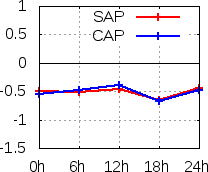
\includegraphics[height=5.5cm]{./figs/VIES850temp0Z.png}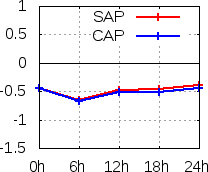
\includegraphics[height=5.5cm]{./figs/VIES850temp12Z.png}
\includegraphics[height=5.5cm]{./figs/EQMtemp0Z.png}\includegraphics[height=5.5cm]{./figs/EQMtemp12Z.png}
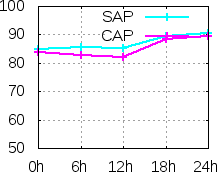
\includegraphics[height=5.5cm]{./figs/CA850temp0Z.png}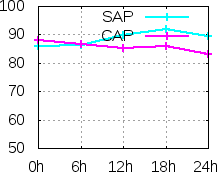
\includegraphics[height=5.5cm]{./figs/CA850temp12Z.png}
\caption{Viés, EQM e CA para a variável temperatura do ar em 850 hPa. A coluna da esquerda mostra os valores das medidas para o horário das 00Z. A coluna da esquerda mostra os valores das medidas para o horário das 12Z.}
\label{fig11}
\end{figure}

A avaliação dos índices estatísticos considerados para a variável temperatura em 850 hPa, su-gere que, no geral, o experimento CAP tende a subestimar mais os valores de temperatura ao longo de 24 horas de previsão, tanto às 00Z quanto às 12Z do que o experimento SAP. Este resultado se reflete diretamente nos valores do EQM, principalmente durante as 12 primeiras horas de previsão. Este resultado pode ser associado ao fato de que há menos observações de temperatura no horário das 00Z do que no horário das 12Z. Outro fator que pode ser associado a este resultado é a dependência de que a precipitação tem dos processos de escala de subgrade, seja na liberação de calor latente ou na modulação do perfil vertical de umidade, o qual a tempe-ratura está associada.

A assimilação de precipitação pelo modelo EtaWS é um processo de inicialização física, onde as variáveis prognósticas do modelo são inicializadas de acordo com as alterações nos perfis verticais de calor e umidade. Estes perfis são alterados quando se compara a precipitação produzida pelo modelo em relação à precipitação observada (conforme explicado no \autoref{assimprec} na \autoref{tab02}). A temperatura é uma das variáveis que são diretamente influenciadas pelas alterações nos perfis de calor e umidade, devido à sua condição de referência no esquema de convecção. 

A CA da temperatura para o horário das 00Z é menor para o experimento CAP nas 12 primeiras horas de previsão e tendem a ser maior nas últimas 12 horas, em comparação ao experimento SAP. No horário das 12Z observa-se o contrário, sendo o experimento CAP melhor do que o experimento SAP nas 12 primeiras horas de previsão.

As \autoref{fig12} e \autoref{fig13}, mostram os valores dos índices de Viés e EQM para a temperatura do ar nos níveis de 500 e 250 hPa. Em médios e altos níveis, observa-se que o viés da temperatura tende a apresentar um comportamento semelhante ao apresentado em baixos níveis, reforçando a idéia de que a temperatura é sensível às alteração de calor e umidade. No entanto, enquanto que em médios níveis, no horário das 12Z o EQM da temperatura tende a ser pequeno, em altos níveis este erro é muito grande e chega a ser uma ordem de grandeza maior. Em geral, observa-se que o experimento CAP subestima menos os valores de temperatura do que o experimento SAP. A CA da temperatura para esses níveis foi omitida por não apresentar resultados relevantes.
 	 
\begin{figure}[!hbp]
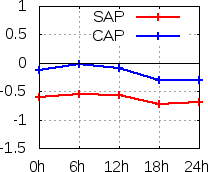
\includegraphics[height=5.5cm]{./figs/VIES500temp0Z.png}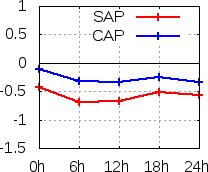
\includegraphics[height=5.5cm]{./figs/VIES500temp12Z.png}
\includegraphics[height=5.5cm]{./figs/EQMtemp0Z.png}\includegraphics[height=5.5cm]{./figs/EQMtemp12Z.png}
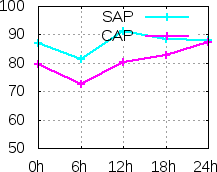
\includegraphics[height=5.5cm]{./figs/CA500temp0Z.png}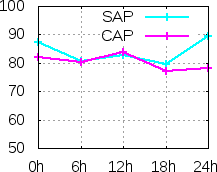
\includegraphics[height=5.5cm]{./figs/CA500temp12Z.png}
\caption{Viés, EQM e CA para a variável temperatura do ar em 500 hPa. A coluna da esquerda mostra os valores das medidas para o horário das 00Z. A coluna da esquerda mostra os valores das medidas para o horário das 12Z.}
\label{fig12}
\end{figure}

\begin{figure}[!hbp]
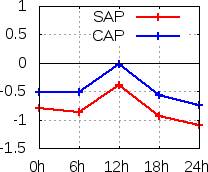
\includegraphics[height=5.5cm]{./figs/VIES250temp0Z.png}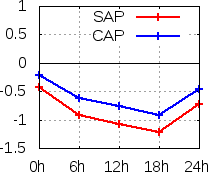
\includegraphics[height=5.5cm]{./figs/VIES250temp12Z.png}
\includegraphics[height=5.5cm]{./figs/EQMtemp0Z.png}\includegraphics[height=5.5cm]{./figs/EQMtemp12Z.png}
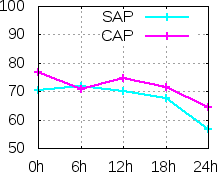
\includegraphics[height=5.5cm]{./figs/CA250temp0Z.png}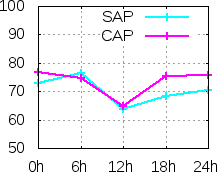
\includegraphics[height=5.5cm]{./figs/CA250temp12Z.png}
\caption{Viés, EQM e CA para a variável temperatura do ar em 250 hPa. A coluna da esquerda mostra os valores das medidas para o horário das 00Z. A coluna da esquerda mostra os valores das medidas para o horário das 12Z.}
\label{fig13}
\end{figure}

\subsection{Estudo de Caso}

Durante o período do projeto SALLJEX, foram identificados em torno de 100 SCMs entre as ba-cias Amazônica e do Prata, no Altiplano Sul-americano. No mês de Janeiro de 2003, ocorreram dois casos de CCM, o primeiro no dia 18 de Janeiro e o segundo no dia 23 de Janeiro. Vários autores (\cite{zipseretal04}; \cite{herdiesetal04}) estudaram estes eventos e outros estudos numéricos foram realizados com o objetivo de simular os CCMs com modelos regionais de mesoescala. \citeonline{paegleetal04} comparam vários modelos regionais, dentre eles versões diferentes dos modelos RAMS, MM5 e Eta (incluindo o modelo regional operacional, na época, do CPTEC Eta 40 km). Os autores mostram que existe uma grande variação entre as previsões dos diferentes modelos e apontam as possíveis causas como sendo condições iniciais e de contorno não muito realistas, dados de baixa qualidade e parametrizações inadequadas. Neste mesmo caso, os autores mostram também, como exemplo, o caso do CCM ocorrido no dia 18 de Janeiro em que os modelos regionais não foram capazes de simular as principais ca-racterísticas do CCM. Em altas resoluções (e.g., 20 km), os modelos regionais são capazes de prever grandes acumulados de precipitação, mas, no entanto, não refletem bem as característi-cas associada aos SCMs. \citeonline{paegleetal04} ainda apontam para o fato de que a inicialização e a validação dos modelos pode beneficiar a análises geradas pelos modelos de previsão.

Para este estudo de caso, foi escolhido o CCM ocorrido no dia 23 de janeiro de 2003. Este CCM foi escolhido pelo fato de também ter sido estudado por outros autores como \citeonline{rozante06}. Além disso, o caso de CCM ocorrido no dia 18 de Janeiro de 2003, também não foi bem caracte-rizado pelos experimentos com assimilação (CAP). Conjectura-se que o modelo EtaWS com o esquema de assimilação de precipitação não tenha sido capaz de caracterizar de forma adequa-da esse caso de CCM devido às suas características dinâmicas, diferentes do segundo caso de CCM, do dia 23 de Janeiro de 2003.
Na \autoref{fig14} são mostradas as imagens do canal 4 (infravermelho) do satélite \textit{Geostationary Satellite Server}  8 (GOES 8). Nestas imagens, observa-se um CCM que começou a se formar no dia 22 de janeiro de 2003 às 18Z, tendo seu ciclo de vida com duração total de um dia, culminado ao dia 23 de janeiro de 2003 às 12Z. Na \autoref{fig15}, é mostrada a precipitação diária observada do SALLJEX, acumulada às 12Z. Na \autoref{fig16}, a precipitação estimada pelo TRMM.

Com as simulações dos experimentos SAP e CAP, buscou-se observar se o modelo de previsão Eta e o sistema de assimilação de dados RPSAS foram capazes de simular esse complexo convectivo. Diante das configurações ajustadas para o modelo de previsão (rodando com e sem a assimilação de precipitação e com filtro digital), e comparando-se o resultado dos experimentos com os dados do SALLJEX e do TRMM, pode-se notar que sem a assimilação de precipitação (experimento SAP), o modelo não foi capaz de reproduzir o evento de precipitação ocasionado pelo CCM. Apenas com a assimilação de precipitação (experimento CAP), o modelo foi capaz de reproduzir a precipitação ocasionada pelo CCM.

Para efeito de comparação, vale lembrar que durante o experimento de campo do SALLJEX, foram instalados vários pluviógrafos adicionais na região de estudo o que favoreceu uma descri-ção muito mais minuciosa dos acumulados de precipitação. A precipitação do TRMM3B42, embora possua uma resolução temporal mais refinada (3 horas), mostra que em seus acumulados uma distribuição de precipitação mais discreta do que a do SALLJEX, principalmente às 06Z do dia 23 de Janeiro de 2003, quando o CCM atinge seu estágio maduro. O campo de precipitação produzido pelo modelo EtaWS , com o experimento CAP, apresenta também taxas de precipitação inferiores àquelas observadas no SALLJEX, embora sua distribuição espacial seja coerente com o que foi encontrado na observação.

\begin{sidewaysfigure}[!hbp]
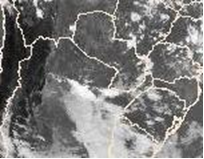
\includegraphics[height=4.3cm]{./figs/sat01.png}\hspace{0.2cm}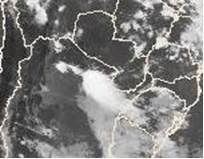
\includegraphics[height=4.3cm]{./figs/sat02.png}\hspace{0.2cm}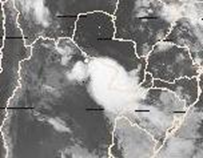
\includegraphics[height=4.3cm]{./figs/sat03.png}\hspace{0.2cm}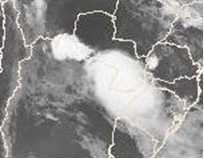
\includegraphics[height=4.3cm]{./figs/sat04.png}
\\[0.15cm]
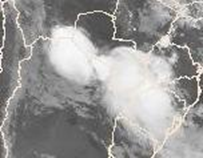
\includegraphics[height=4.3cm]{./figs/sat05.png}\hspace{0.2cm}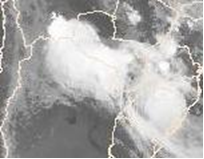
\includegraphics[height=4.3cm]{./figs/sat06.png}\hspace{0.2cm}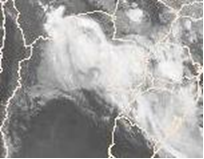
\includegraphics[height=4.3cm]{./figs/sat07.png}\hspace{0.2cm}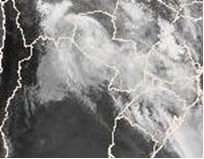
\includegraphics[height=4.3cm]{./figs/sat08.png}
\caption{Imagens do Satélite GOES 8 no canal 4 (infravermelho). Evolução de um complexo convectivo de mesoescala. Nas figuras: (a) 20030122$\_$18Z; (b) 20030122$\_$21Z; (c) 20030123$\_$00Z; (d) 20030123$\_$03Z; (e) 20030123$\_$06Z; (f) 20030123$\_$09Z; (g) 20030123$\_$12Z; (h) 20030123$\_$15Z.}
\label{fig14}
\end{sidewaysfigure}

\begin{sidewaysfigure}[!hbp]
\centering
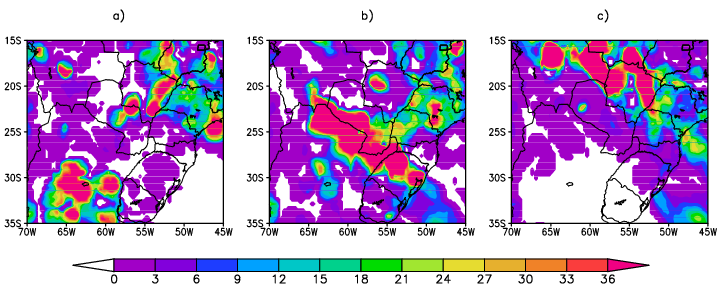
\includegraphics[height=7.9cm]{./figs/prec_salljex.png}
\caption{Precipitação observada diária SALLJEX, acumulado 12Z. Nas figuras: a) 20030122$\_$12Z; b) 20030123$\_$12Z; c) 20030124$\_$12Z.}
\label{fig15}
\end{sidewaysfigure}

Observando-se as imagens do canal infravermelho do GOES 8, nota-se que o CCM começou a se formar às 18Z do dia 22 de Janeiro e atinge o seu estágio maduro (o máximo de precipitação) às 06Z do dia 23, quando observa-se os critérios de forma tamanho e tempo de duração definidos por \citeauthoronline{maddox80} para a caracterização do CCM.

\begin{sidewaysfigure}[!hbp]
\centering
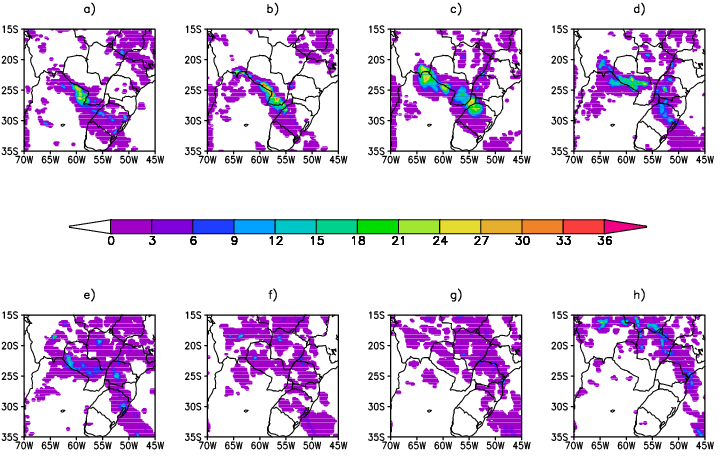
\includegraphics[height=12.2cm]{./figs/prec_trmm.png}
\caption{Precipitação Estimada (TRMM3B42). Evolução de um complexo convectivo de mesoescala. Nas figuras: a) 20030123$\_$00Z; b) 20030123$\_$03Z; c) 20030123$\_$06Z; d) 20030123$\_$09Z; e) 20030123$\_$12Z; f) 20030123$\_$15Z; g) 20030123$\_$18Z; h) 20030123$\_$21Z.}
\label{fig16}
\end{sidewaysfigure}

As imagens da \autoref{fig16} mostram a precipitação estimada do TRMM correspondentes às imagens de satélite do GOES 8.

\begin{sidewaysfigure}[!hbp]
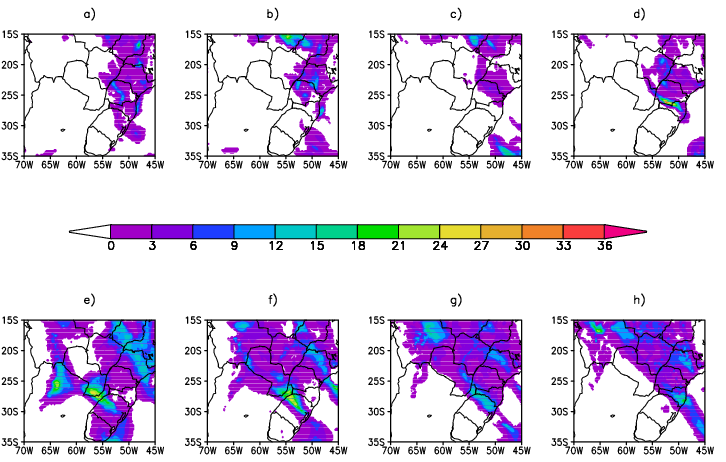
\includegraphics[height=12.2cm]{./figs/prec_eta.png}
\caption{Precipitação Prevista pelo sistema Eta+RPSAS a partir do dia 22/01/003. Nas figuras: previsões de a) 6h; b) 12h; c) 18h e d) 24h para o experimento SAP, e) 6h; f) 12h; g) 18h e h) 24h para o experimento CAP.}
\label{fig17}
\end{sidewaysfigure}

Nota-se que 6 horas após (09Z do dia 23) o máximo de precipitação do CCM (06Z do dia 23), embora o CCM ainda apresente suas características principais, a precipitação do TRMM apre-senta taxas relativamente menores do que o observado pelo SALLJEX no acumulado das 12Z do dia 23. 

Os campos de precipitação produzidos pelo modelo EtaWS com os experimentos SAP e CAP, mostram diferenças significativas durante as previsões de 6, 12, 18 e 24 horas. A assimilação dos dados de precipitação fez com que o modelo EtaWS reproduzisse de forma satisfatória o campo de precipitação apresentado na imagem ``c'' da \autoref{fig16}. No entanto, levando-se em consideração os esquemas físicos do modelo,  a melhor discretização dos tipos de solo do mo-delo de superfície NOAH e o esquema de convecção BMJ, nota-se também que as simulações do experimento CAP tendem a superestimar e a espalhar um pouco mais a precipitação nos horários subsequentes à 06Z do dia 23 de Janeiro.

A próxima \autoref{fig18} mostra os perfis verticais do vento meridional entre os níveis de 1000 hPa e 250 hPa. Nesta figura são mostrados os perfis de vento para os dois experimentos testados (SAP e CAP) e o perfil de vento da Reanálise 2 do NCEP/DOE para a latitude de 22ºS (próximo à localidade de Mariscal no Paraguai - não mostrado) onde ocorreu o CCM. 

\begin{figure}[!hbp]
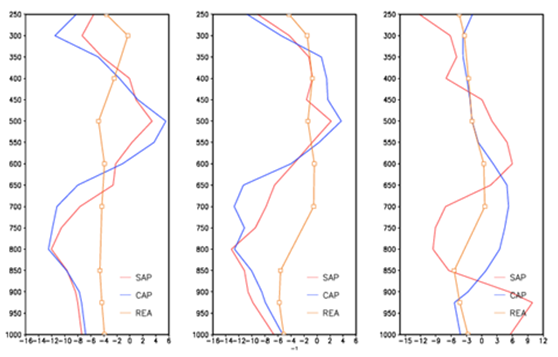
\includegraphics[height=9.8cm]{./figs/perfilvento.png}
\caption{Perfis do vento meridional na latitude de 22ºS, próximo à localidade de Mariscal. Em amarelo a Reanálise 2 do NCEP/DOE, em azul o experimento CAP e em vermelho o experimento SAP. Na imagem da esquerda: 18Z do dia 22 de Janeiro. Na imagem do centro: 00Z do dia 23 de Janeiro e na imagem da direita, as 06Z do dia 23 de Janeiro. Unidades estão em m/s.}
\label{fig18}
\end{figure}

Os perfis de vento meridional mostram nos horários anteriores à ocorrência do CCM, os dois experimentos (SAP e CAP) mostravam-se concordantes quanto à intensidade, superestimando a intensidade apresentada pelo vento da reanálise. Já no horário referente ao estágio de maturação do CCM (às 06Z do dia 23), observa-se que o experimento SAP coloca o vento no sentido contrário do que é apresentado pela reanálise e pelo experimento CAP. \citeonline{herdies06} apresenta os mesmos perfis de vento meridional para a latitude de 22ºS juntamente com as observa-ções de vento do SALLJEX. Os resultados apresentados pelo experimento CAP concordam em direção e intensidade (do vento) com o que foi simulado pelos modelos globais do NCEP.

A \autoref{fig19} mostra a seção vertical do fluxo de umidade também para a latitude de 22ºS. Nesta figura são mostrados os resultados encontrados para os experimentos SAP (primeira linha) e CAP (segunda linha). Nesta figura nota-se que o fluxo de umidade apresentado pelo experimento CAP às 06Z do dia 23 apresenta valores elevados (da ordem de 100 g/kg m/s).

\begin{figure}[!hbp]
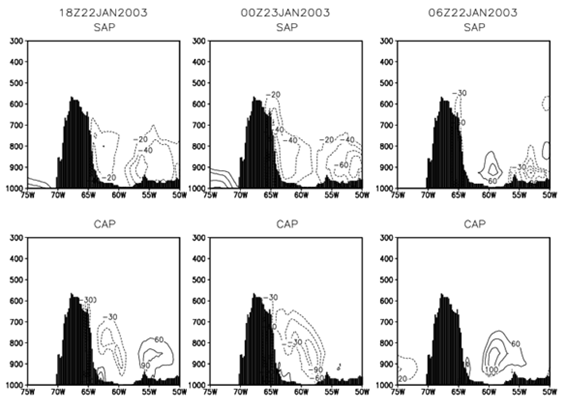
\includegraphics[height=11cm]{./figs/secvert.png}
\caption{Seção vertical do fluxo de umidade ($qv$) ao longo da latitude de 22ºS, às 18Z do dia 22 (coluna da esquerda), às 00Z do dia 23 (coluna do meio) e às 06Z do dia 23 de Janeiro. Os contornos estão em g/kg m/s.}
\label{fig19}
\end{figure}

A \autoref{fig20} mostra os campos de velocidade vertical (Omega) em 700 hPa para os experimen-tos SAP e CAP e a precipitação do SALLJEX. Comparando-se os dois experimentos, nota-se que o experimento CAP foi capaz de detalhar melhor o desenvolvimento vertical das nuvens convectivas associadas ao CCM. Os contornos em azul-claro representam valores de -0.2 Pa/s. Em \citeonline{herdies06} estes valores são de -0.5 Pa/s. Levando-se em consideração que não foram assimilados dados do SALLJEX nos experimentos SAP e CAP.
 
\begin{figure}[!hbp]

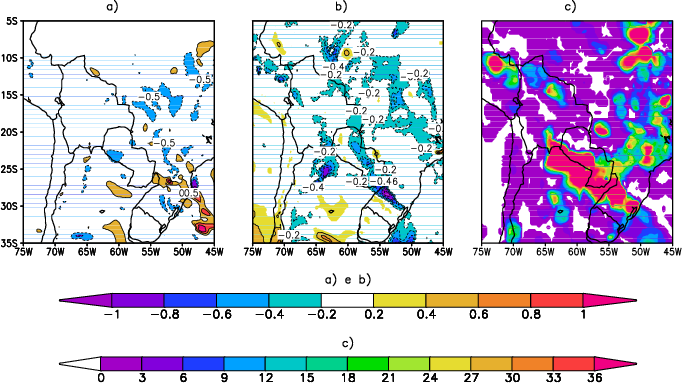
\includegraphics[height=7cm]{./figs/omega.png}
\caption{Velocidade vertical em 700 hPa para os experimentos a) SAP e b) CAP. Em ambos os casos são mostradas as previsões de 6 horas. Em c) precipitação observada do SALLJEX. Os contornos em azul-claro apresentam valores iguais a -0.2 Pa/s.}
\label{fig20}
\end{figure}
